% !TeX root = ../main.tex

\chapter{移动操作机器人的系统搭建}
\label{cha:system}


\section{机械结构设计}

按结构划分,可以将Tinker的机械结构粗略的划分为头部,机械臂,骨架,身体主控
以及底盘。机器人的整体外观如图~\ref{fig:tinker_front_side}所示。

\begin{figure}[ht] % use float package if you want it here
  \centering
  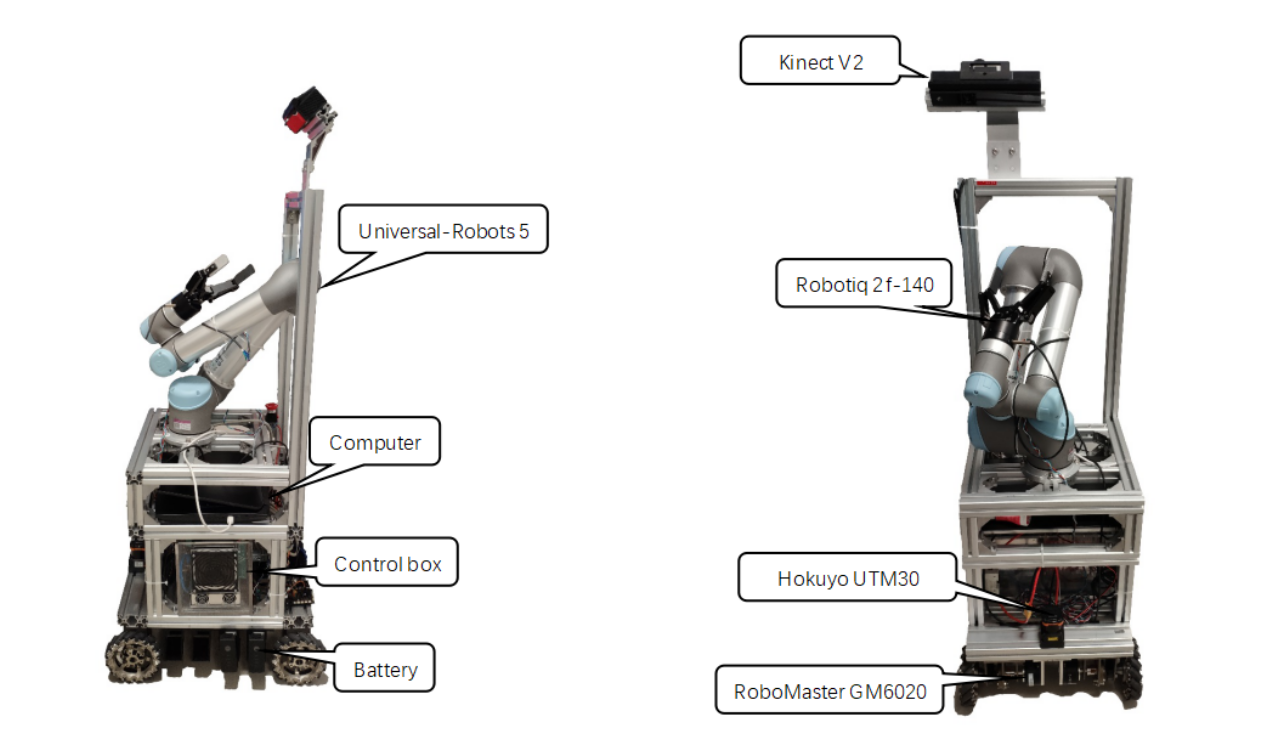
\includegraphics[width=1.\linewidth]{tinker_front_side.png}
  \caption{Tinker前视图与侧视图}
  \label{fig:tinker_front_side}
\end{figure}

\subsection{Tinker骨架搭建}
为方便交通运输与结构迭代,Tinker基本骨架使用40cm*40cm铝形材搭建。骨架
的主要作用为搭建起整个机器人的框架,将各个传感器假设到理想的位置上,并且
为机器人的主控、供电、走线留出足够的空间。经过多轮版本迭代后,目前Tinker
底盘尺寸固定在35cm×45cm,净高140cm,总质量70kg。

为了方便Tinker机器人机械结构长期的维护,降低人员交接成本,我们将Tinker
使用的型材尺寸做了规范化处理,并且对骨架进行了手动建模,以方便机器人的拆
装与改进,如图~\ref{fig:base_link}所示。

\begin{figure}[ht] % use float package if you want it here
  \centering
  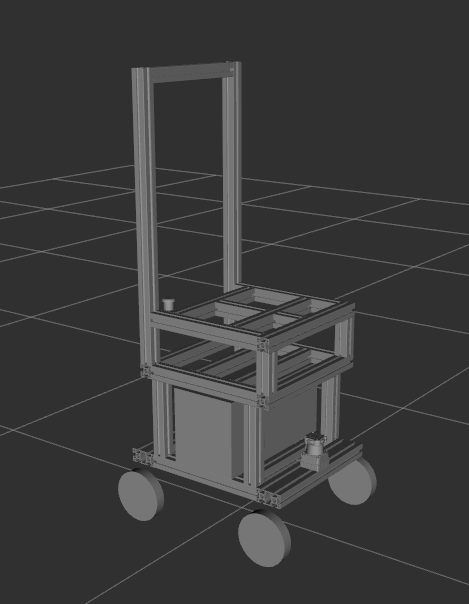
\includegraphics[width=.4\linewidth]{base_link.png}
  \caption{Tinker骨架的STL建模结果}
  \label{fig:base_link}
\end{figure}

\subsection{头部设计及版本迭代}

新版的Tinker头部主要用来放置顶部摄像头,在背景环境特别复杂的情况下还会在头部
旁边加装专业的采音麦克风用于语音识别和声源定位。在一般情况下使用头部安装的kinect v2
摄像头自带的麦克风阵列即可满足需求。在Tinker中期我们曾经使用过2自由度云台支持
头部摄像头,使头部摄像头具有上下和左右转动的能力,以扩大摄像头的视野,如图~\ref{fig:neck}
所示。该转台是机器人团队根据现有的通用二自由度转台自行改装的,主要改动有:更换了
原有的舵机,改为精度更高且有位置反馈的dynamixel MX28-AR舵机,
并且相应的改装了转台本身的尺寸和各种装配零件。客观上这一设计确实提高了机器人头部
传感器的视野,但是经过漫长的实践,这一结构被证明是一个彻头彻尾的失败设计。原因有
二:dynamixel本身需要合理的供电和信号线,摄像头本身也有相应的传输线,这些线在频繁
转动的时候很容易被拉断造成整个控制系统崩溃;摄像头本身作为抓取和部分避障的主力
传感器,其位置精度是非常重要的,但是由于舵机空程以及装配过程中产生的空程等等问题,
转台的位置精度一直无法达到要求,大大减弱了摄像头的数据效果。因此在新版的Tinker
中,转台这一设计被机器人团队彻底抛弃了。

\begin{figure}[ht] % use float package if you want it here
  \centering
  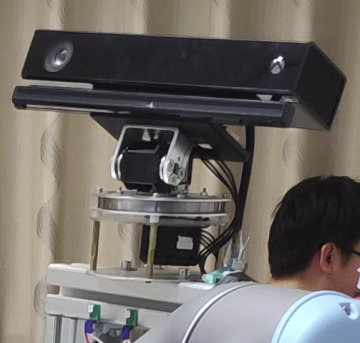
\includegraphics[width=.4\linewidth]{neck.png}
  \caption{早期Tinker头部的2自由度转台}
  \label{fig:neck}
\end{figure}

\subsection{Tinker机械臂方案选择}

Tinker使用的机械臂为Universal Robotics公司生产的6自由度机械臂UR5。在决定使用
该机械臂之前我们对市面上在售的各种成品机械臂进行了广泛的调研,包括RoboCup@Home
赛场上使用过的Kinova~\ref{fig:kinova}
机械臂配合三指夹爪,Retinker Robotics公司开发的Sawyer(图~\ref{fig:sawyer})
机械臂,以及Universal Robotics公司出产的各个型号的机械臂(图~\ref{fig:ur_series})。
最终综合考虑了价格、售后、供电、开发者社区等
各个因素后,我们最终确定使用了UR5这个型号的机械臂,并且对机械臂的控制与供电进行了
适当的改装,以符合比赛的需要。

\begin{figure}
\centering
\begin{subfigure}{.5\textwidth}
  \centering
  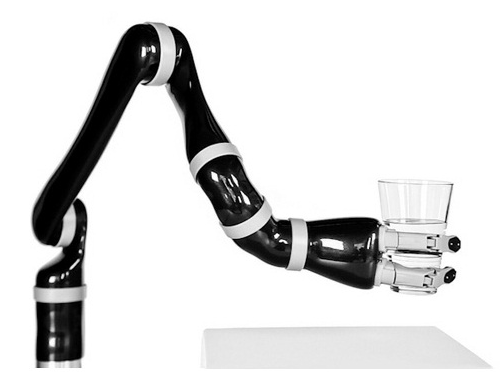
\includegraphics[width=.9\linewidth]{kinova.png}
  \caption{Kinova}
  \label{fig:kinova}
\end{subfigure}%
\begin{subfigure}{.5\textwidth}
  \centering
  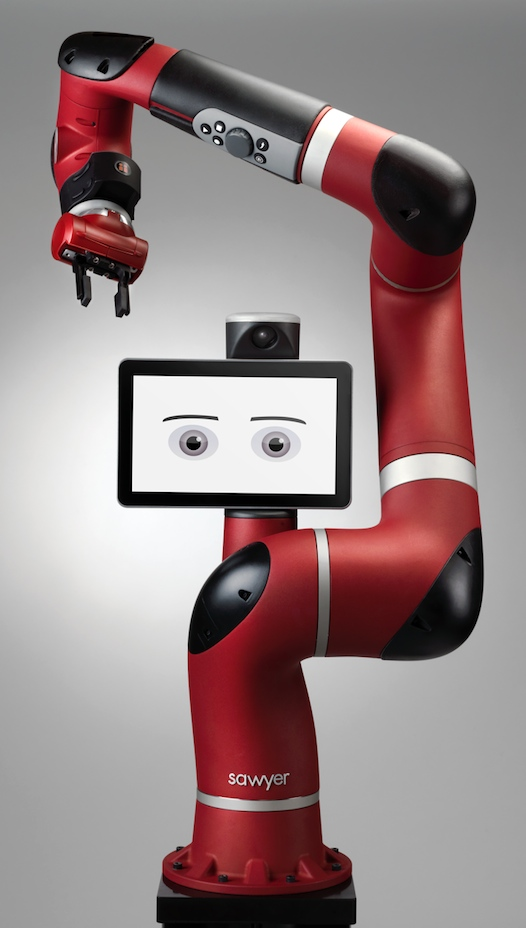
\includegraphics[width=.5\linewidth]{sawyer.jpg}
  \caption{Sawyer}
  \label{fig:sawyer}
\end{subfigure}
\begin{subfigure}{.8\textwidth}
  \centering
  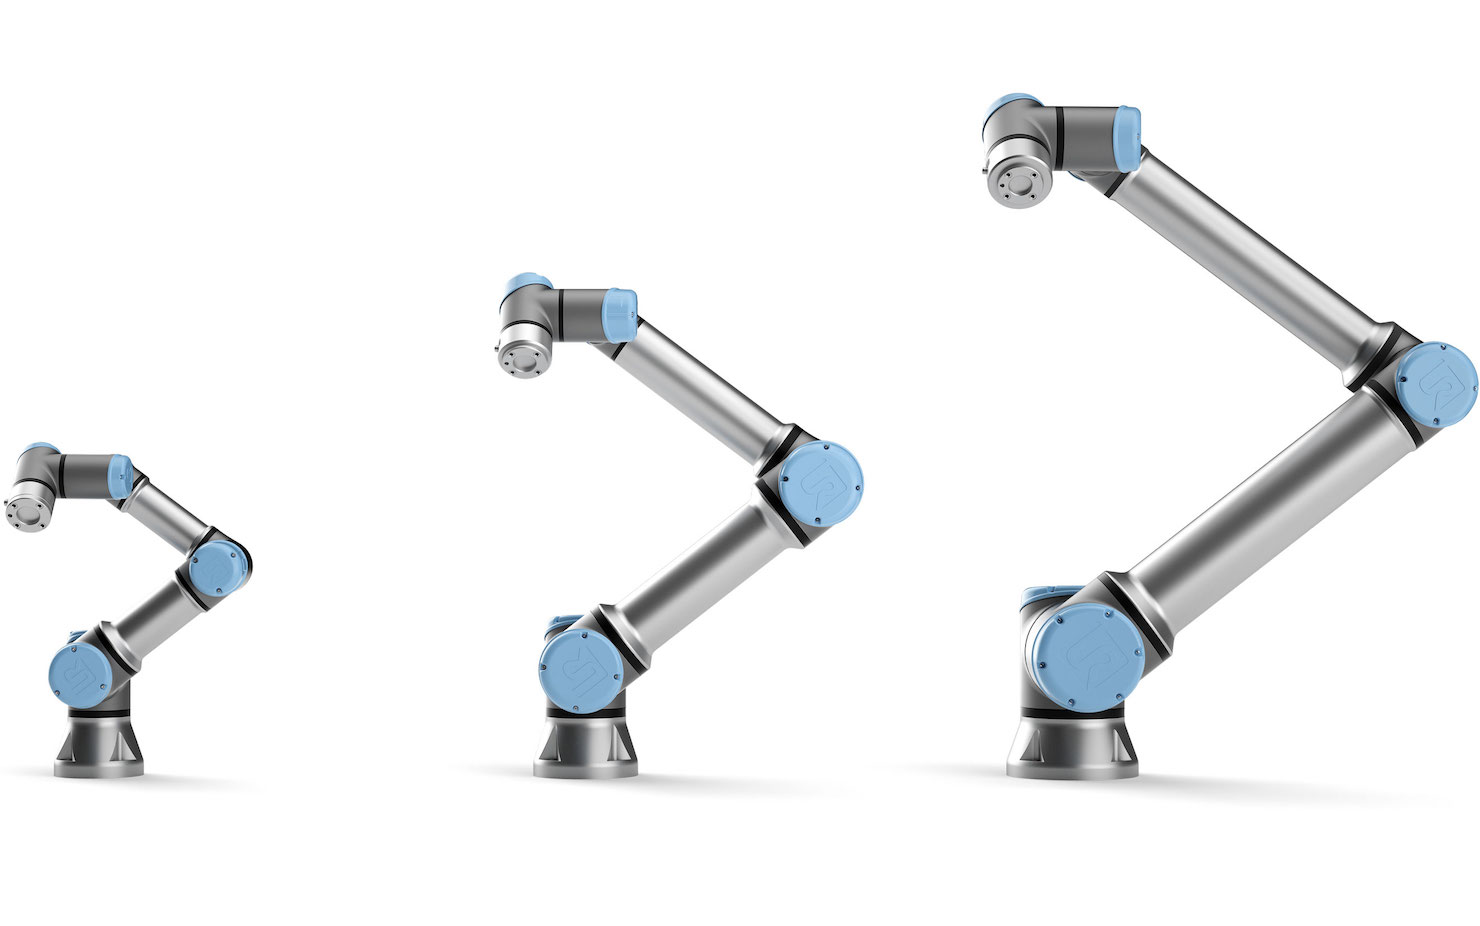
\includegraphics[width=.7\linewidth]{ur_series.jpg}
  \caption{UR系列机械臂}
  \label{fig:ur_series}
\end{subfigure}
\caption{本工作前期调研时关注过得机械臂型号}
\label{fig:arms}
\end{figure}

早期夹爪使用Robotiq
公司生产的Robotiq 2f-85二指夹爪(最大张角85mm),后经过不断的测试与赛场上的较量,
我们发现2f-85的张角对于家庭机器人来说过窄,于是换用了robotiq 2f-140款式的二指夹爪,
该夹爪张角为140mm,能够更好的满足抓取物品、拾取袋子的需求。因此本工作最终使用
UR5 + Robotiq 2f-140作为最终比赛方案,如图~\ref{fig:ur5_2f140}所示。

\begin{figure}[ht] % use float package if you want it here
  \centering
  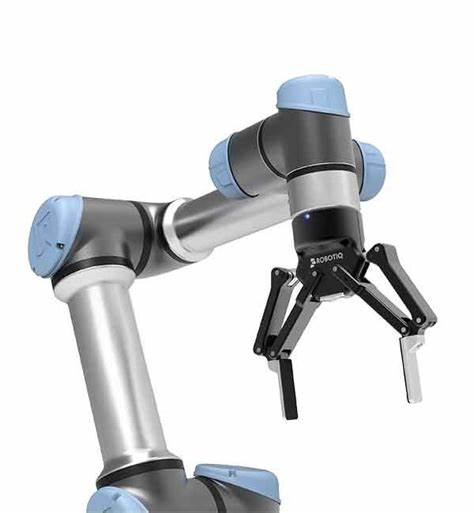
\includegraphics[width=.4\linewidth]{ur5_2f140.jpeg}
  \caption{Tinker最终使用的机械臂及夹爪方案}
  \label{fig:ur5_2f140}
\end{figure}

\subsection{主控与供电}

Tinker的核心控制由一台搭载了i9-9900K cpu及RTX2080显卡的笔记本电脑完成。在前
几代Tinker设计中,一般主控由工控机或者经过电源改装的台式机担任,但是随着笔记本
性能的不断增强,我们最终选择使用成品机器完成这一任务。成品笔记本性能好,散热完善
且主板设计精良,稳定性好,并且笔记本有自己独立的供电系统,可在机器人断电时单独运行
大大的提升了系统的稳定性和易用性。

整个机器人的供电系统都放在机器人腹部,包括机械臂、底盘、各种传感器、笔记本电脑所需
的所有供电电路以及电池组。2019年Tinker使用单一磷酸铁锂电池供电,标准输出电压29.4V
到24V,容量50AH,放在底盘上部。经过19年比赛的反思之后,作者认为,使用单一锂电池
供电太过危险,且参赛过程中运输太过麻烦,成本过高,于是我们将供电方案改成了多块标准
29V 1500mAH电池并接供电的形式,并3D打印了特制的电池架将电池倒挂在底盘下,这样一方面
大大缩小了Tinker底盘的面积提高了底盘避障导航的灵活性,另一方面降低了整个机器人的中心,
使得机械臂运动时的型变更小,提高了机器人的性能。在供电电路布线方面,Tinker也有了
显著的改进,前一版本中Tinker直接借用了UR5自带的配电箱摆放机械臂及其他部件需要的
供电线路、DCDC、分流排等等元件。但是配电箱本身尺寸过大,不透明,且强度过大,给机器人
装配、调试带来了很大的困难,也对导航的表现造成了影响。之后我们在充分考虑了散热、消防
等等制约之后,使用亚克利版重新制作了一版配电箱,且对机器人的供电线路进行了梳理,大大
缩小了机器人的底盘尺寸,也使得整个供电设计更加简洁易于调试。前后两个版本的供电外观
如图~\ref{fig:elec}所示。

\begin{figure}
\centering
\begin{subfigure}{.5\textwidth}
  \centering
  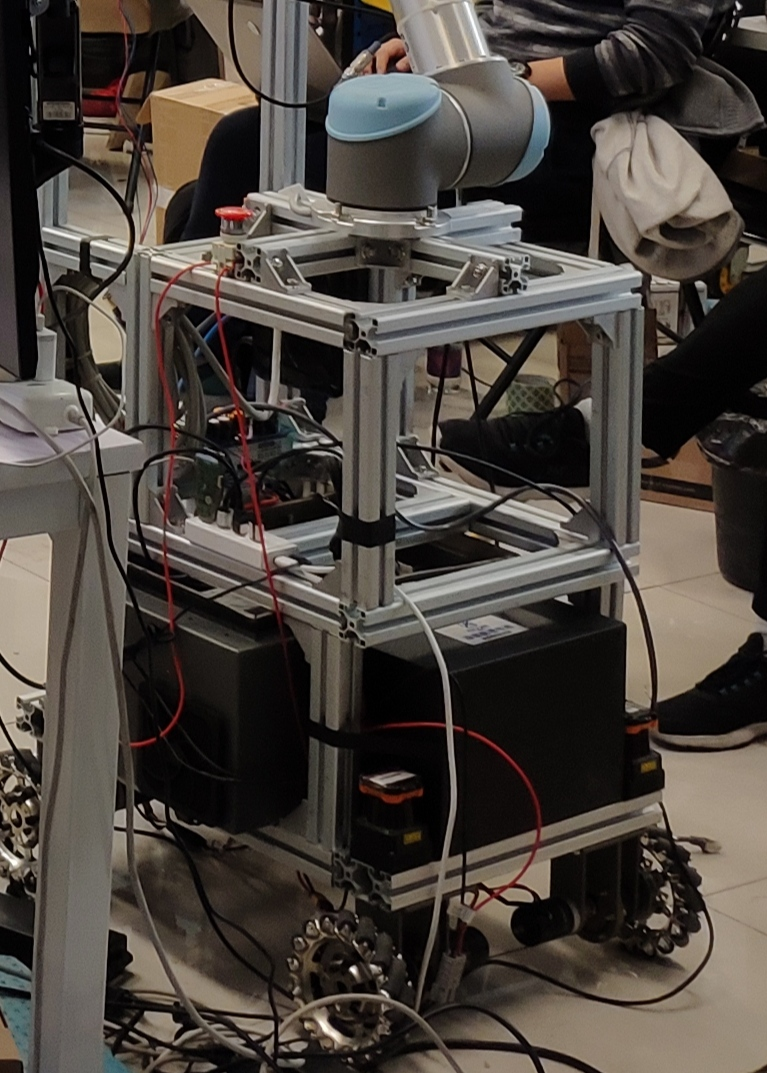
\includegraphics[height=6cm]{tinker_elec.jpg}
  \caption{改版前的电池及供电线路放置}
  \label{fig:old_elec}
\end{subfigure}%
\begin{subfigure}{.5\textwidth}
  \centering
  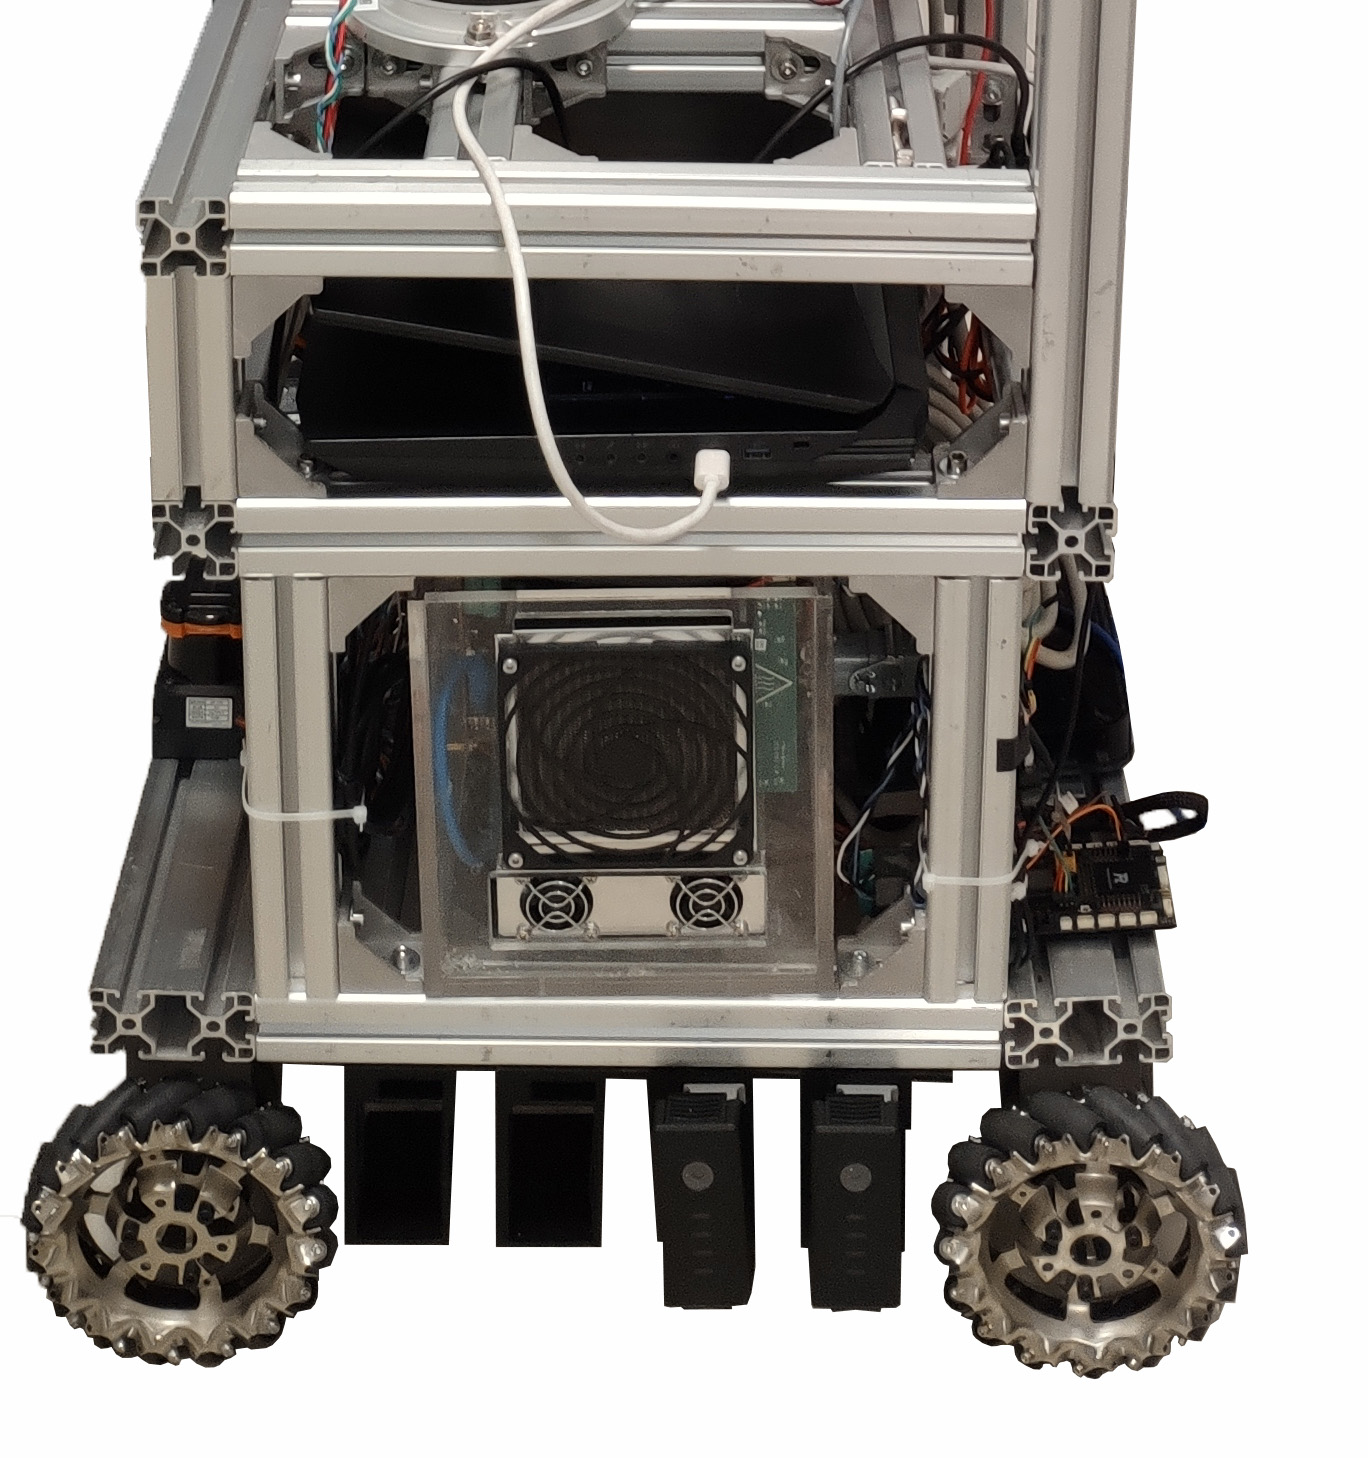
\includegraphics[height=6cm]{tinker_elec_new.jpg}
  \caption{改版后的电池及供电线路放置}
  \label{fig:new_elec}
\end{subfigure}
\caption{Tinker前后两个版本的供电布局}
\label{fig:elec}
\end{figure}

\subsection{底盘设计}

Tinker的底盘设计受前几版机器人的影响最多,早期的Tinker使用自制的3自由
度机械臂,其精度有限且自由度受限太严重,需要具有左右额外自由度的底盘
来弥补这一不足,因此Tinker的底盘被设计为使用4个麦克纳母轮的万向底盘
\cite{tlale2008kinematics},底盘设计如图~\ref{fig:chassis_sw}所示,
由于我们使用的麦轮为标准成品,因此在设计图中将麦轮的细节全部简化了。

\begin{figure}[ht] % use float package if you want it here
  \centering
  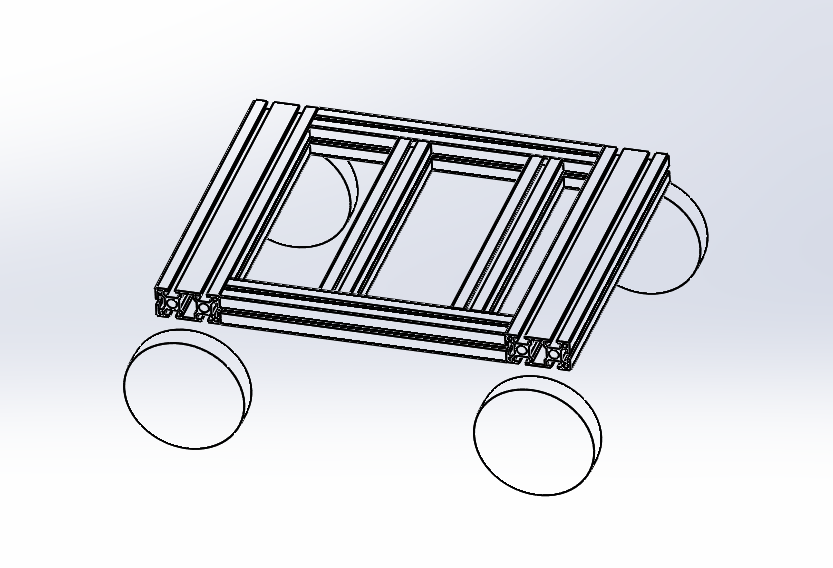
\includegraphics[width=.7\linewidth]{chassis_sw.png}
  \caption{Tinker底盘悬架的SolidWorks设计图}
  \label{fig:chassis_sw}
\end{figure}

新版Tinker改为成品机械臂后抓取的自由度和覆盖范围都有了质的飞跃,不再要求
底盘具有万向移动的性能了。但是经过多年的改进,机器人团队中对万向底盘的制作
技术已经成熟,于是我们继续沿用了这一设计,仅在电机选型上做了一些与时俱进
的改良,选用了扭矩较大且噪音较小的大疆 GM6020直流无刷电机做底盘的动力电机,
如图~\ref{fig:chassis}所示。

\begin{figure}[ht] % use float package if you want it here
  \centering
  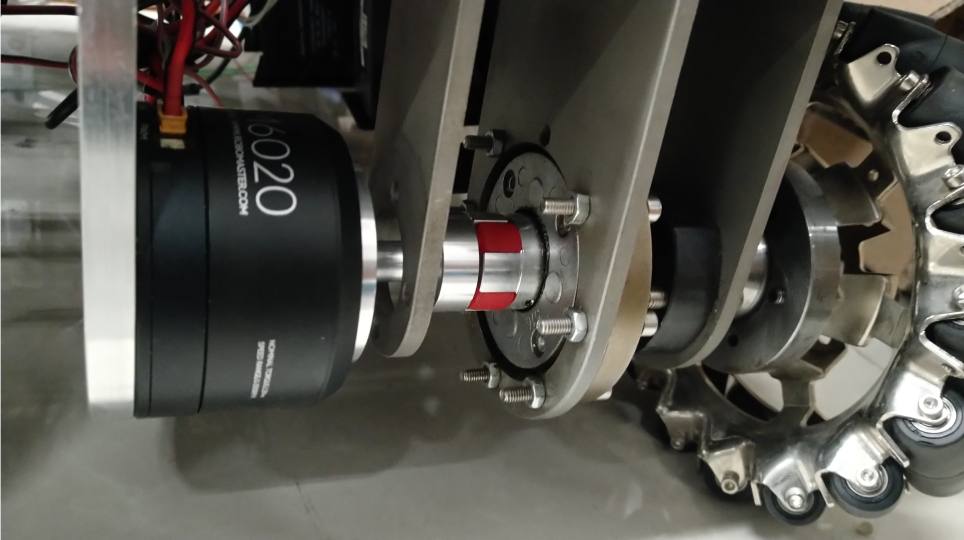
\includegraphics[width=.7\linewidth]{chassis.png}
  \caption{Tinker底盘的电机传动结构}
  \label{fig:chassis}
\end{figure}


\section{电路设计及通信设计}

Tinker机器人作为一个有复杂功能和结构的完整机器人系统,经过长时间的开发
和改进,其控制电路及各个部件之间的通信是及其复杂的。经过不断的实验和试错,
本工作创造性的将软件设计中分定义接口、分层描述的概念引入到机器人
的硬件设计中,对机器人的供电、通信均给出了清晰详尽的分层描述。这一描述大大
的方便了各部分之间的分工协作,提高了开发的效率。

\subsection{供电系统设计及演化}

新版Tinker在搭建之初由于时间紧迫,使用一台逆变器将电池输出的29V直流电源
经过一台逆变器直接转到220V交流电(图~\ref{fig:dc_ac}所示),再连接各个
执行控制部件与传感器。在一段
时间内,这个方案虽然丑陋,但很好的满足了机器人的任务需求,为Tinker机器人的发展
作出了贡献。但是这个方案的缺陷也非常明显,逆变器本身效率很低,且体积不小,
再加上市电转到各个传感器的开销,整个机器人变得异常臃肿,且续航极短。逆变器
工作时还会发出高频啸叫,对机器人的安全和性能都有严重损害。

经过一段时间的调研,作者对Tinker的供电系统做了2次系统的改造,逐步的将
供电改为直流直接供电,并且理顺了机器人内部的供电逻辑。其供电分层描述如图~\ref{fig:charge}
所示

\begin{figure}[ht] % use float package if you want it here
  \centering
  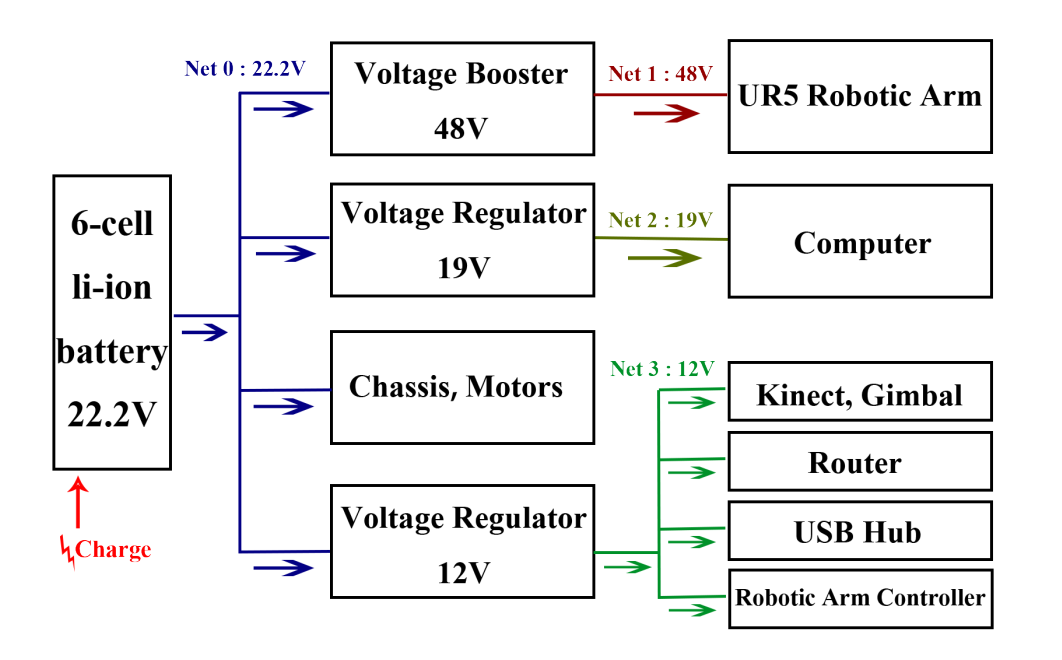
\includegraphics[width=.7\linewidth]{charge.png}
  \caption{Tinker的分层供电示意图}
  \label{fig:charge}
\end{figure}

在供电改造的过程中,最消耗精力的是UR5机械臂的供电改造。UR5机械臂本身所需
的功率极大且其本身的保护机制过于复杂,在机械臂上电时有一套复杂的自检逻辑,
会在直流供电端尝试拉取一个十几A的大电流对电源进行冲击检测,并且在电流拉取
结束后还会反复切断电路进行电源测试。这一逻辑过于复杂,市面上常用的DC-DC
普遍无法满足需求。本文作者经过长时间的反复测试和大量的文献检索,最终
使用明纬SD-1000L-48V开关电源(图~\ref{fig:sd1000l_48}所示)替代普通
电源对机械臂单独供电才满足机械臂的
供电改造需求。

\begin{figure}
\centering
\begin{subfigure}{.5\textwidth}
  \centering
  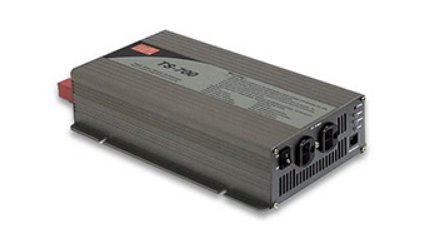
\includegraphics[width=.6\linewidth]{dc_ac.png}
  \caption{明纬TS-700-248B 700W逆变器}
  \label{fig:dc_ac}
\end{subfigure}%
\begin{subfigure}{.5\textwidth}
  \centering
  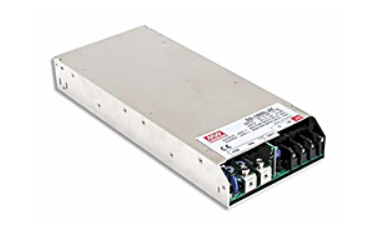
\includegraphics[width=.7\linewidth]{sd1000l_48.png}
  \caption{明纬SD-1000L-48V开关电源}
  \label{fig:sd1000l_48}
\end{subfigure}
\caption{Tinker电路改造中使用过的供电元件}
\label{fig:charge_hareware}
\end{figure}

概括的说,Tinker的供电系统中有4个主要电压,分别是电池直接输出且底盘直接
使用的22.2V,机械臂
工作电路需要的48V,笔记本电脑充电需要的19V,各个传感器、路由器以及机械臂
主控需要的12V电压。除机械臂供电使用了明纬SD1000L-48开关电源外,其他变压
需求均使用了一般市售的大功率直流DCDC电源。在经过两轮改版后,Tinker的供电
系统以基本稳定,目前Tinker整机上电待机时长能达到1.5h左右,高负荷运行时(
机械臂高负荷运行且同时执行高强度计算任务,或者底盘不间断运行)可连续工作
20分钟左右,基本满足比赛需求。

\subsection{通信系统设计}

由于Tinker使用了大量的成品部件,包括机械臂、夹爪、电机、各种传感器等等,
其通信设计受限比较大。机器人团队使用开源且在机器人科研领域广泛的ROS框架完成
高层数据及控制通信,辅以必要的底层通信控制,完成整个系统的数据获取与命令
执行功能,其分层设计示意图如~\ref{fig:communication}所示。

\begin{figure}[ht] % use float package if you want it here
  \centering
  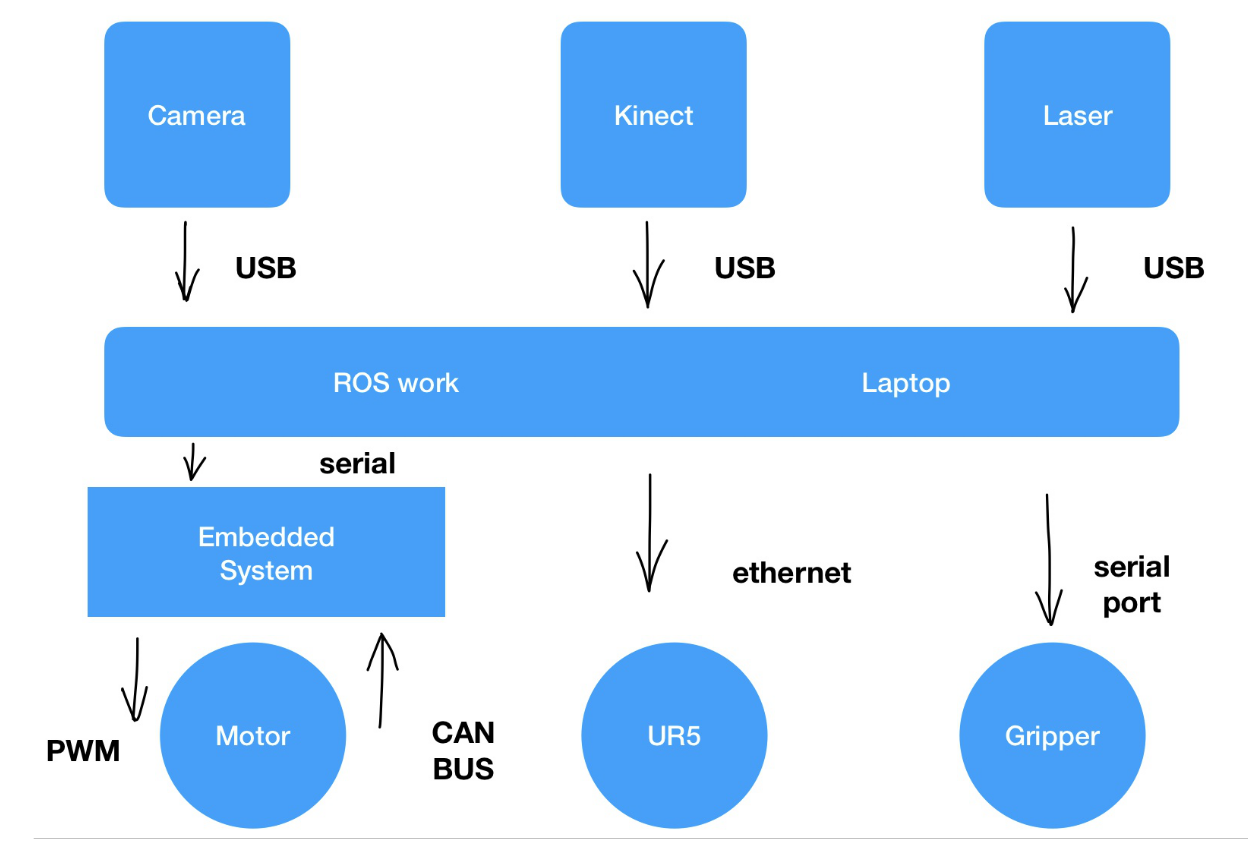
\includegraphics[width=.7\linewidth]{communication.png}
  \caption{Tinker的分层通信示意图}
  \label{fig:communication}
\end{figure}

头部Kinect、激光雷达及额外的摄像头(一般安装在机械臂腕部,为一台realsense d435)
通过usb直接连接到中央控制电脑上,通过ros驱动打开,获取的数据流直接发布到
ROS的通信系统中,夹爪使用串口同样连接到电脑上,使用ROS驱动进行控制。UR5
机械臂本身有主控机器,它通过路由器于中央控制电脑连接,两者利用ROS的ethernet
通讯机制通信。麦轮底盘的四个电机统一使用CAN总线连接到一块STM32F4单片机
开发板上,开发板通过PWM控制电机转动,电机内部的编码器数据通过CAN回传到
单片机中,单片机再通过串口与主控电脑通信,为了方便底盘接入Tinker的通信
系统,我们使用rosserial对单片机的串口进行封装,完成控制底盘、获取底盘数据
的功能。


\section{本章小结}

本章详细给出了多模态移动操作机器人Tinker的系统搭建信息,对其结构、供电、电子、
通信、控制原理均给出了详细的设计原理和描述。对关键的部件给出了准确的型号信息,
并且详细的描述了部分结构的迭代信息。

下一章本文将主要讲述移动操作机器人软件开发中的重要技术——移动定位与导航技术,
给出目前定位与导航技术的现状,并且详细描述Tinker机器人的方案选择与方案迭代。









